\begin{pycode}

\end{pycode}

\section{Séance 2 - Fréquence de résonance et fonction de transfert}


\subsection{Objectifs}
La première séance de ce projet a permis les observations suivantes :
\begin{itemize}
    \item La fréquence idéale du système se situe à 6.78 MHz (Figure \ref{fig: S}).
    \item À la fréquence de 2.6 MHz, la résistance étant constante en fonction de la position,
    il est difficile d'avoir un capteur de position avec ce système.
    \item Au-delà de la fréquence de 2.6 MHz, le modèle théorique devient trop différent de la réalité.
    \item À une fréquence proche de 150 kHz, pour l'inductance et la résistance, il est possible
    de considérer qu'entre deux positions, le système se comporte de manière linéaire.  
\end{itemize}

\vspace{0,2cm}

Le but de cette séance sera donc d'abaisser la fréquence de résonance du système à une valeur
exploitable. L'abaissement de la fréquence de résonance se fait par la mise en parallèle d'une 
capacité.

\begin{figure}[H]
    \centering
    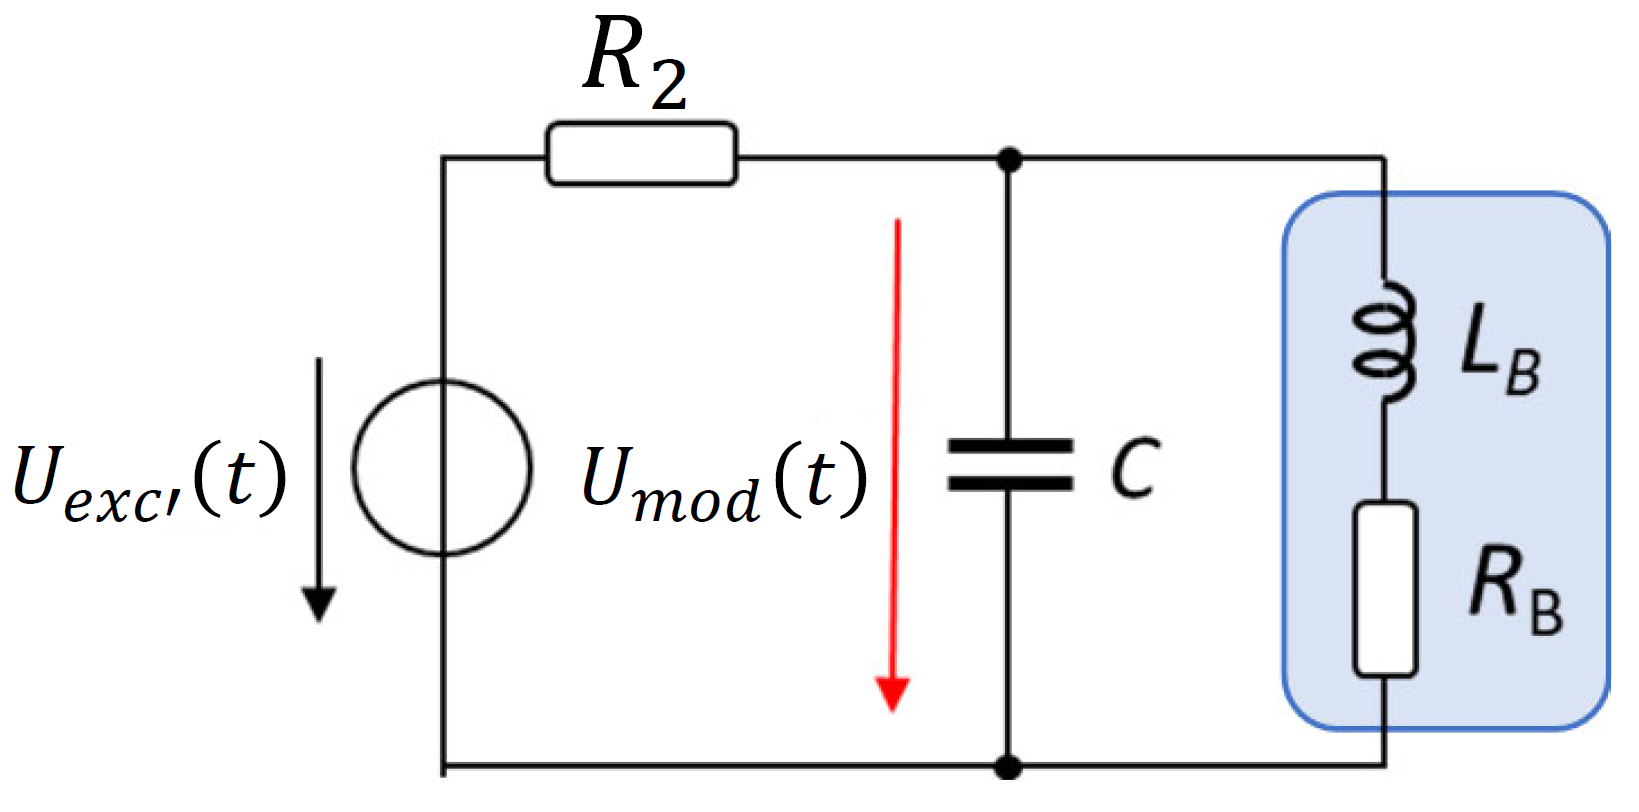
\includegraphics[width=10cm]{Images/Seance2/Circuit_resonant.png}
    \caption{Schéma du circuit résonant}
    \label{fig:circ_res}
\end{figure}
\vspace{0,2cm}

Cette capacité $C$ étant fournie, la fréquence de résonance sera déterminée théoriquement puis par
manipulation. Enfin, une résistance sera ajoutée pour maximiser la sensibilité du système. 



\subsection{Théorie}
\subsubsection{Signal d'excitation}
Le signal d'excitation est un signal carré, de fréquence $f$ et d'amplitude $A$. Par décomposition
en série de Fourrier, ce signal peut être exprimé comme suit :

\begin{equation*}
U_{exc}(t) = \frac{4}{\pi} A \cdot [\sin(\omega \cdot t)+\frac{1}{3}\sin(3\cdot\omega \cdot t)+\frac{1}{5}\sin(5\cdot\omega \cdot t)+...]     
\end{equation*}
\vspace{0,2cm}

Le signal $U_{exc}(t)$ est traité par un filtre passe-bande RLC, conservant uniquement la première
harmonique. Le signal d'excitation devient donc :

\begin{equation*}
    U_{exc'}(t) = \frac{4}{\pi} A \cdot \sin(\omega \cdot t)
\end{equation*}

Ce signal sera celui appliqué à la maquette.

\subsubsection{Fréquence de résonance}

La fréquence de résonance est donnée par l'équation suivante :

\begin{equation*}
    f_0 = \frac{\omega_0}{2\pi} = \sqrt{\frac{1}{L_B\cdot C}-\frac{R_B^2}{L_B^2}}
\end{equation*}

Avec $L_B$ l'inductance de la bobine, $R_B$ sa résistance et C la capacité de précision.
\vspace{0,2cm}

Lors du calcul, il est important de prendre en compte que $L_B$ et $R_B$ dépendent de la fréquence.
Cette équation est donc implicite et nécessite une itération et une interpolation des données pour
calculer la fréquence de résonance.


\subsubsection{Optimisation de la sensibilité}

Pour un circuit en parallèle, la sensibilité à la position de repos et à la fréquence de résonance
est maximisée lorsque $R_0$ est égale à $R_P$.

\begin{figure}[H]
    \centering
    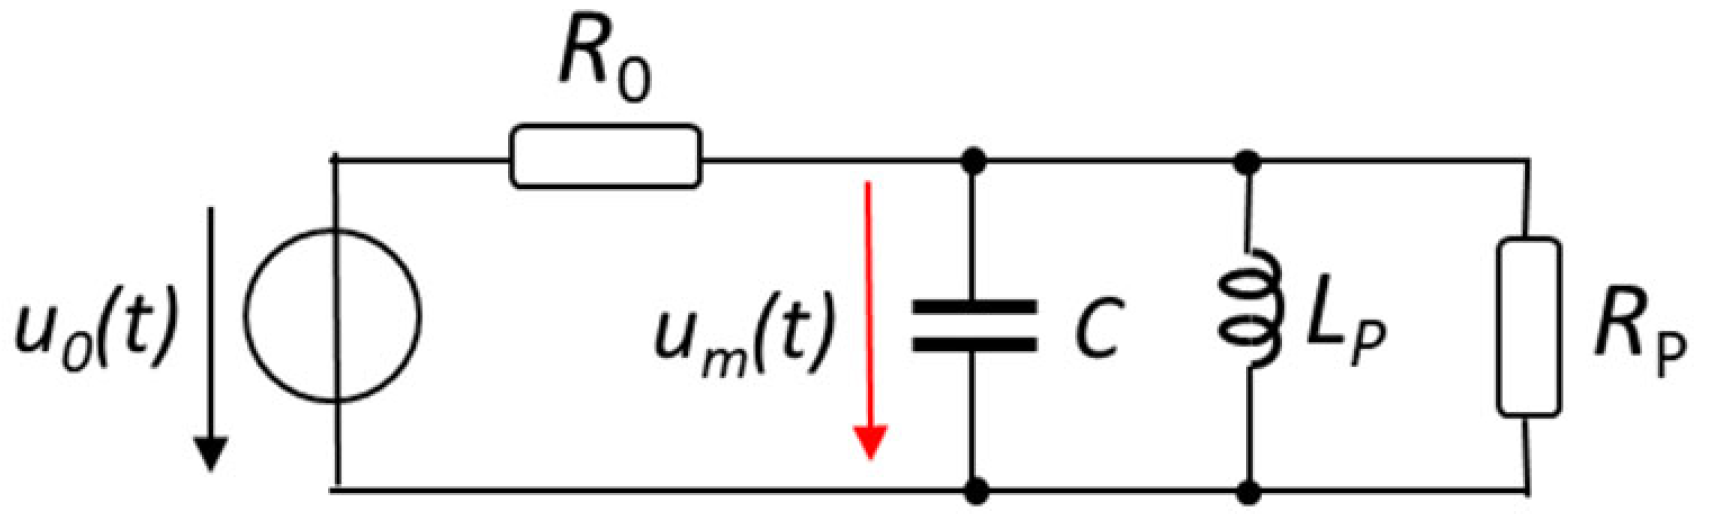
\includegraphics[width=10cm]{Images/Seance2/Circuit_para.png}
    \caption{Schéma du circuit résonant parallèle}
    \label{fig:circ_res_para}
\end{figure}

\vspace{0,2cm}

En effet, à la fréquence de résonance, la capacité et l'inductance peuvent être ignorées. Le système
se comporte alors comme un diviseur résistif.
\begin{figure}[H]
    \centering
    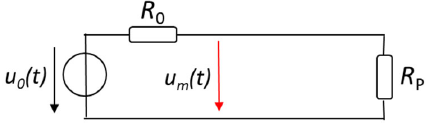
\includegraphics[width=10cm]{Images/Seance2/Circuit_ressss.png}
    \caption{Schéma du circuit résonant parallèle}
    \label{fig:circ_ressss}
\end{figure}

Il est donc possible d'écrire l'équation suivante :

\begin{equation*}
    U_m(t) = \frac{R_P}{R_0+R_P}U_0(t)= \frac{1}{2}U_0(t)
\end{equation*}
Pour notre système :
\begin{equation*}
    U_m(t) = \frac{2}{\pi} A \cdot \sin(\omega \cdot t) 
\end{equation*}

Ce qui donne en valeur crête :

\begin{equation*}
    U_m(t) = \frac{2}{\pi} A 
\end{equation*}

Le système utilisé ayant sa résistance et son inductance en série, il convient de les transformer en
parallèle. La conversion est régie par les équations suivantes :

\begin{equation*}
    L_P = L_B \cdot (1+ \frac{1}{Q^2})
\end{equation*}
\begin{equation*}
    R_P = R_B \cdot (1 + Q^2)
\end{equation*}
\begin{equation*}
    Q = \frac{\omega_0\cdot L_B}{R_B}
\end{equation*}

\subsubsection{Fonction de transfert}
La fonction de transfert du système est donnée par l'équation suivante :
\begin{equation*}
    \underbar{H}(\underbar{$Z_b$}) = \frac{\underbar{$Z_b$}}{(1+j\cdot\omega \cdot C \cdot R_0)\underbar{$Z_b$}+R_0}
\end{equation*}

\subsection{Pratique}
\subsubsection{Matériel}
\begin{figure}[H]
    \centering
    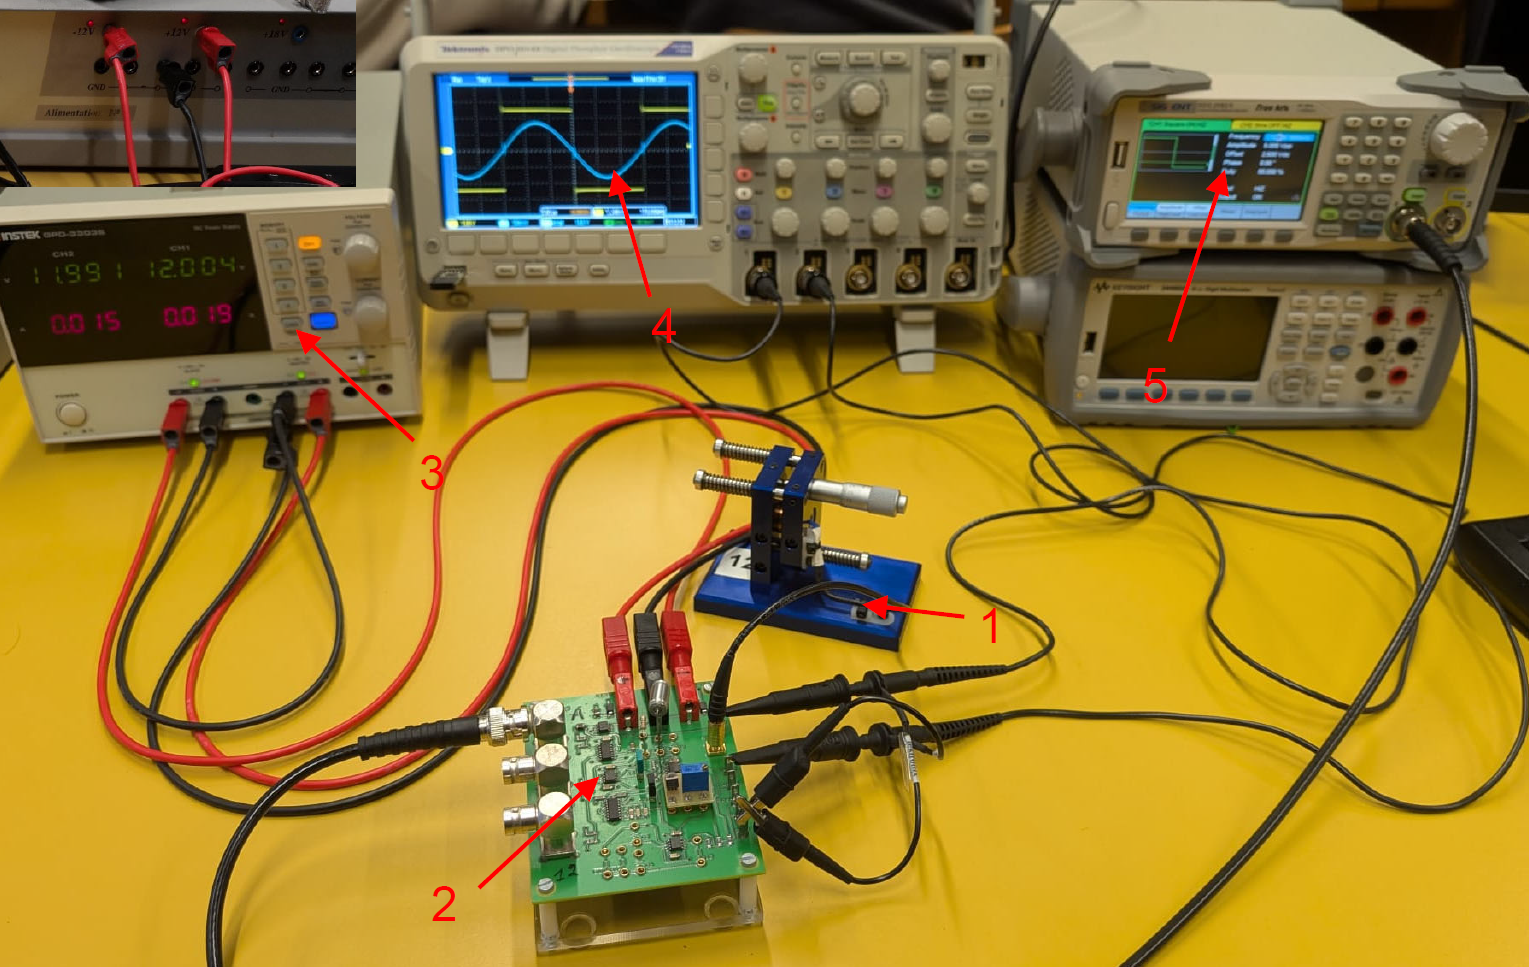
\includegraphics[width=15cm]{Images/Seance2/Montage.png}
    \caption{Montage}
    \label{fig:montage}
\end{figure}
\begin{enumerate}
    \item Maquette
    \item Carte électronique
    \item Alimentation
    \item Oscilloscope
    \item Générateur de signaux
\end{enumerate}

La sonde 1 est sur le signal d'excitation de la carte ($U_{exc}$), la sonde 2 est sur la sortie du
système ($U_{mod}$)


\subsubsection{Fréquence de résonance}
Pour rechercher la fréquence de résonance, la capacité de précision a été montée sur l'emplacement C2.
De plus, une résistance de 820 $\Omega$ a été montée sur l'emplacement R2.
\begin{figure}[H]
    \centering
    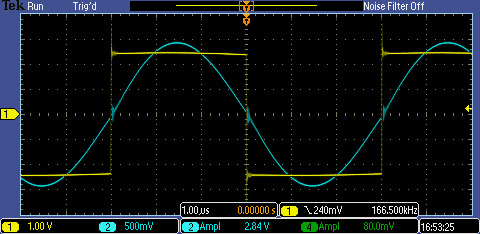
\includegraphics[width=10cm]{Images/Seance2/TEK00000.PNG}
    \caption{Recherche de la fréquence de résonance}
    \label{fig:freq_oscillo}
\end{figure}

\subsection{Résultats}

\subsection{Analyse}

\subsection{Conclusion}
